\documentclass[12pt,spanish]{article}
\usepackage[spanish]{babel}
\usepackage{graphicx}
\usepackage{multirow}
\usepackage{float}
\usepackage{enumitem}
\usepackage[hidelinks]{hyperref}
\usepackage{array}
\graphicspath{ {../img/}}
\usepackage[table]{xcolor}
\selectlanguage{spanish}
\usepackage[utf8]{inputenc}
\usepackage{graphicx}
\usepackage[ddmmyy]{datetime}
\usepackage[a4paper,left=3cm,right=2cm,top=2.5cm,bottom=2.5cm]{geometry}
\makeindex

\begin{document}
\begin{titlepage}

\newlength{\centeroffset}
\setlength{\centeroffset}{-0.5\oddsidemargin}
\addtolength{\centeroffset}{0.5\evensidemargin}
\thispagestyle{empty}

\noindent\hspace*{\centeroffset}\begin{minipage}{\textwidth}

\centering

\includegraphics[width=0.9\textwidth]{logo_ugr.jpg}\\[1.4cm]

\textsc{ \Large Fundamentos de Ingeniería del Software\\[0.2cm]}
\textsc{GRADO EN INGENIERÍA INFORMÁTICA}\\[1cm]

{\Large\bfseries Práctica 3. Análisis y especificación de requisitos\\
}
\noindent\rule[-1ex]{\textwidth}{3pt}\\[3.5ex]
{\normalsize\bfseries Primera parte}
\end{minipage}

\vspace{2.5cm}
\noindent\hspace*{\centeroffset}
\begin{minipage}{\textwidth}
\centering

\textbf{Autores}\\ {José Baena Cobos \\ José Miguel Pelegrina Pelegrina\\Carlos Sánchez Páez}\\[2.5ex]

\includegraphics[width=0.3\textwidth]{etsiit_logo.png}\\[0.1cm]
\vspace{1.5cm}

\includegraphics[width=0.2\textwidth]{lsi.png}\\[0.1cm]
\vspace{1cm}
\textsc{Escuela Técnica Superior de Ingenierías Informática y de Telecomunicación}\\
\vspace{1cm}
\textsc{Curso 2017-2018}
\end{minipage}
\end{titlepage}
\tableofcontents
\thispagestyle{empty}
\listoffigures
\newpage
\setcounter{page}{1}
%%%%%%%%%%%%%%%%%%%%%%%%Comienzo del documento%%%%%%%%%%%%%%%%%%%%%%%%%%%%%%%

\section{Modelo Conceptual}

\begin{figure}[H]
\centering
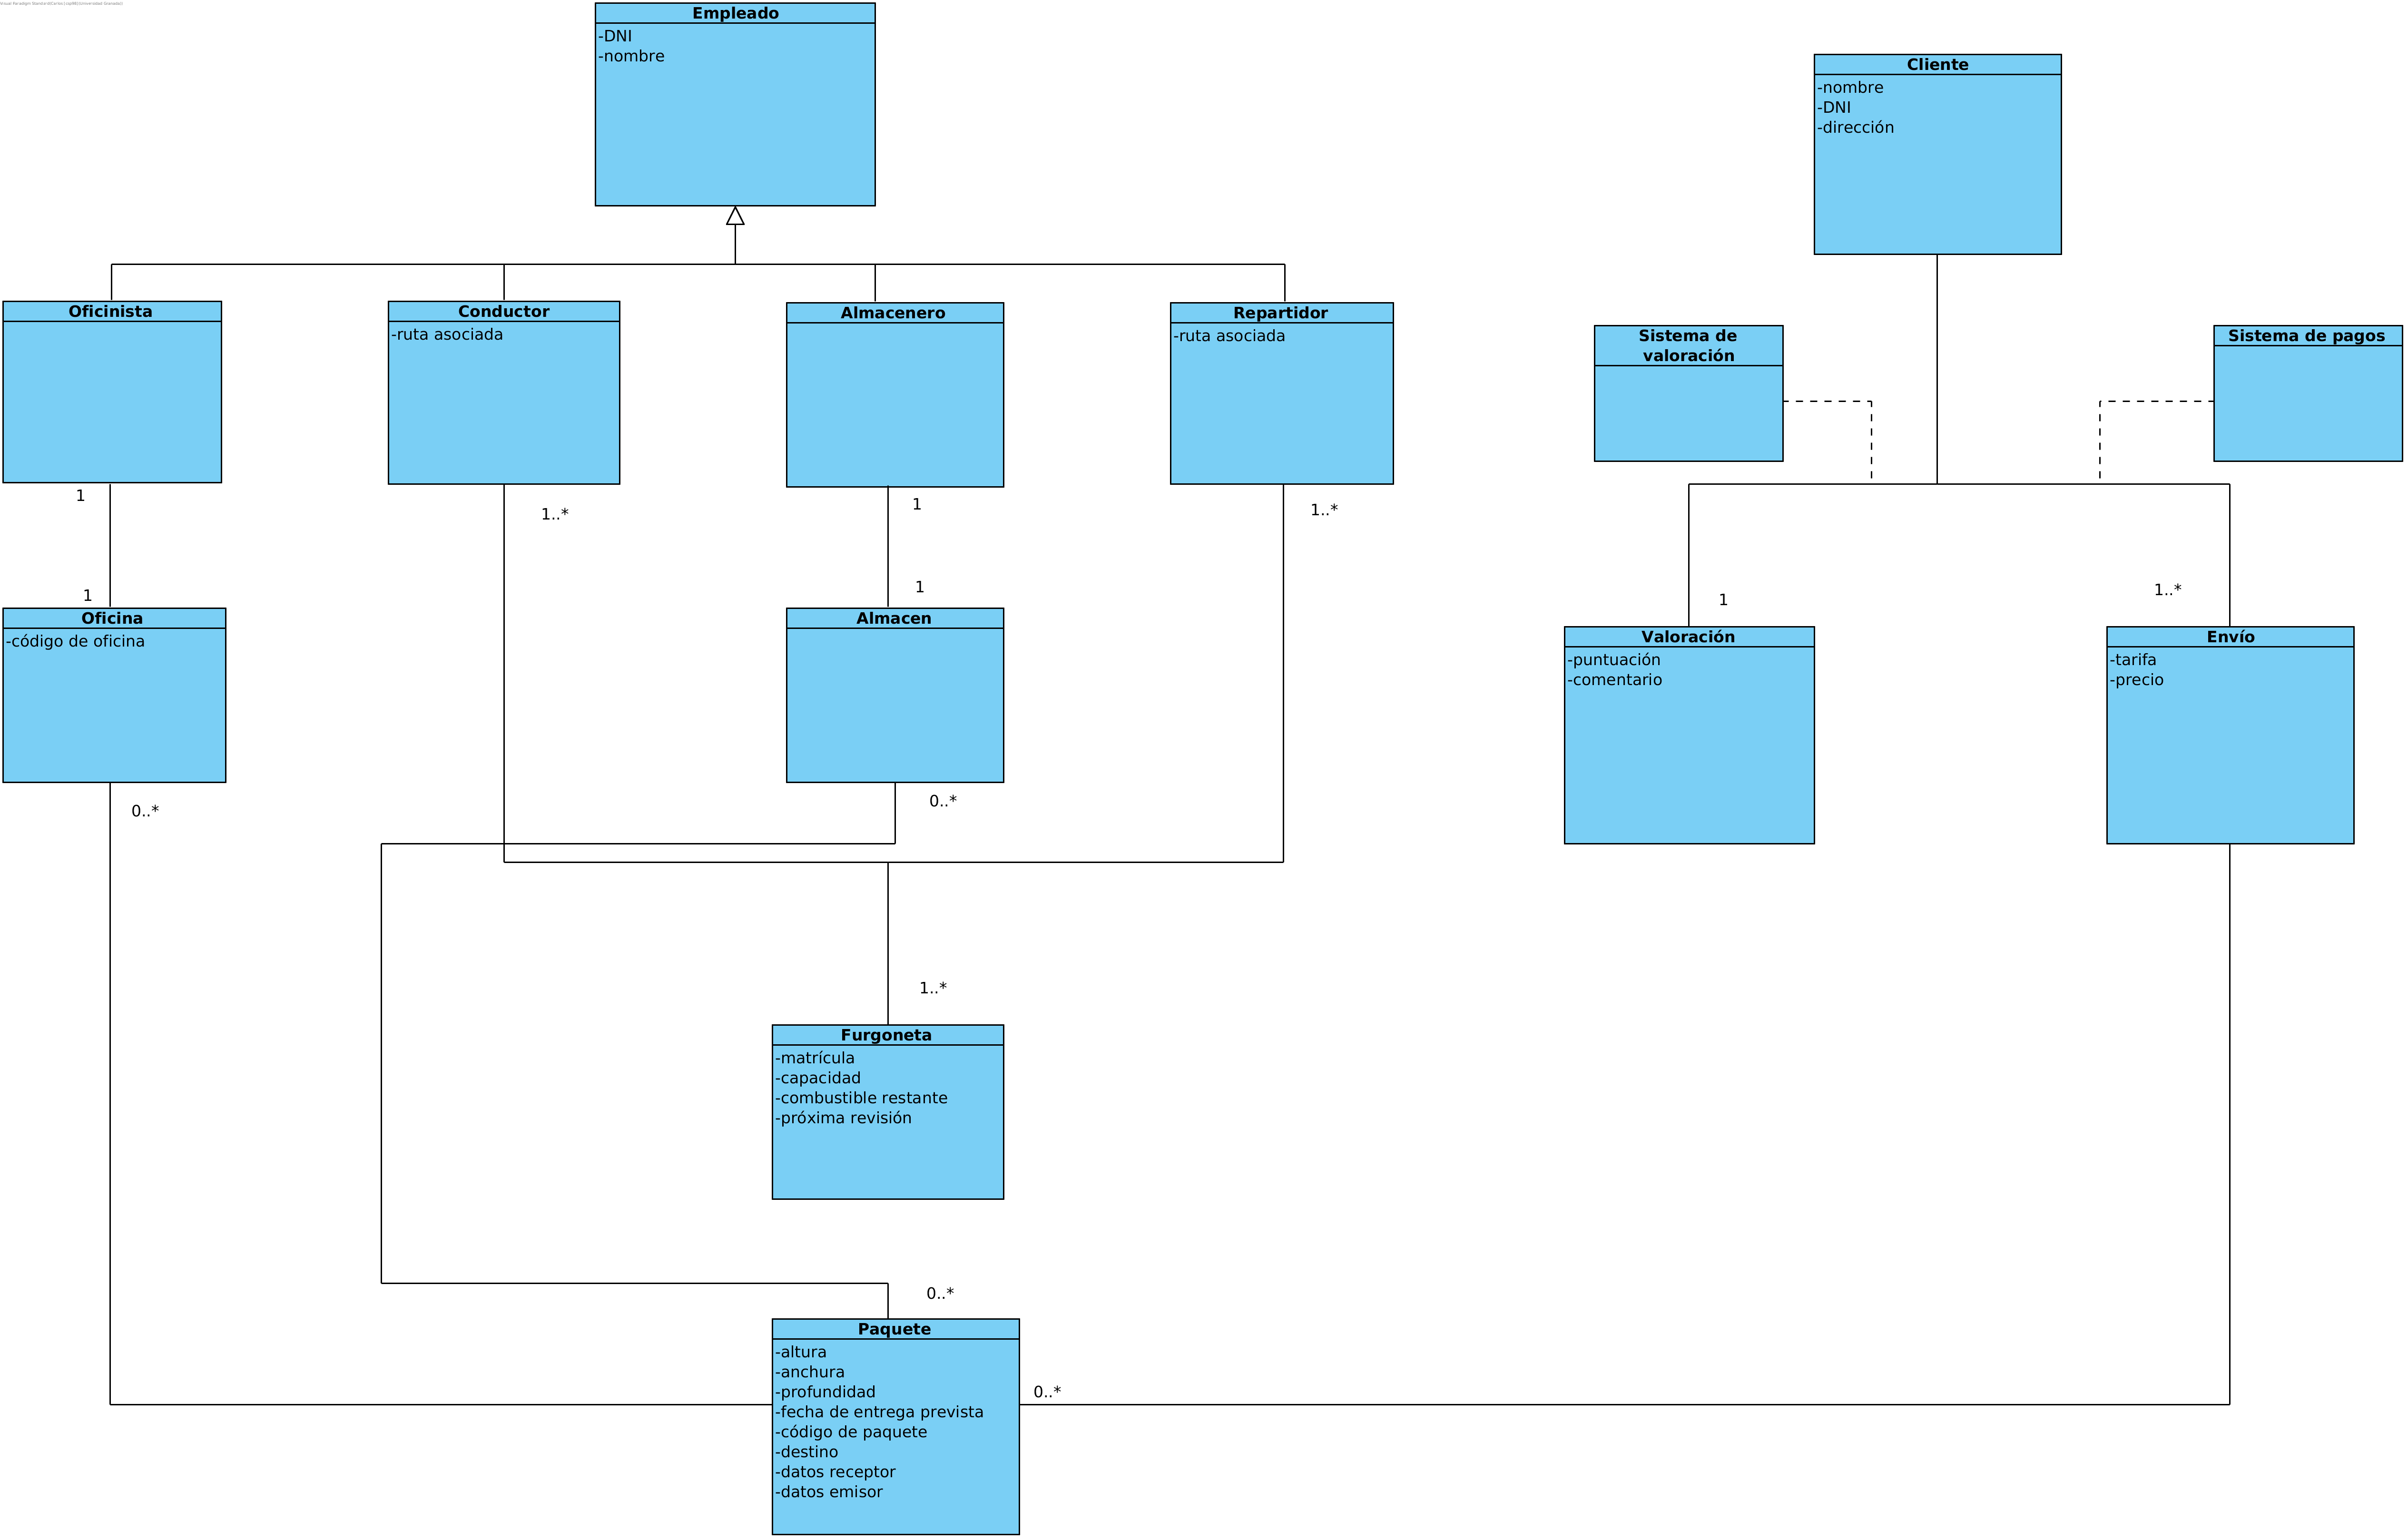
\includegraphics[scale=0.35]{modelo_conceptual.png}
\caption{Modelo conceptual.}
\end{figure}

\section{Diagramas de secuencia}

\begin{figure}[H]
\centering
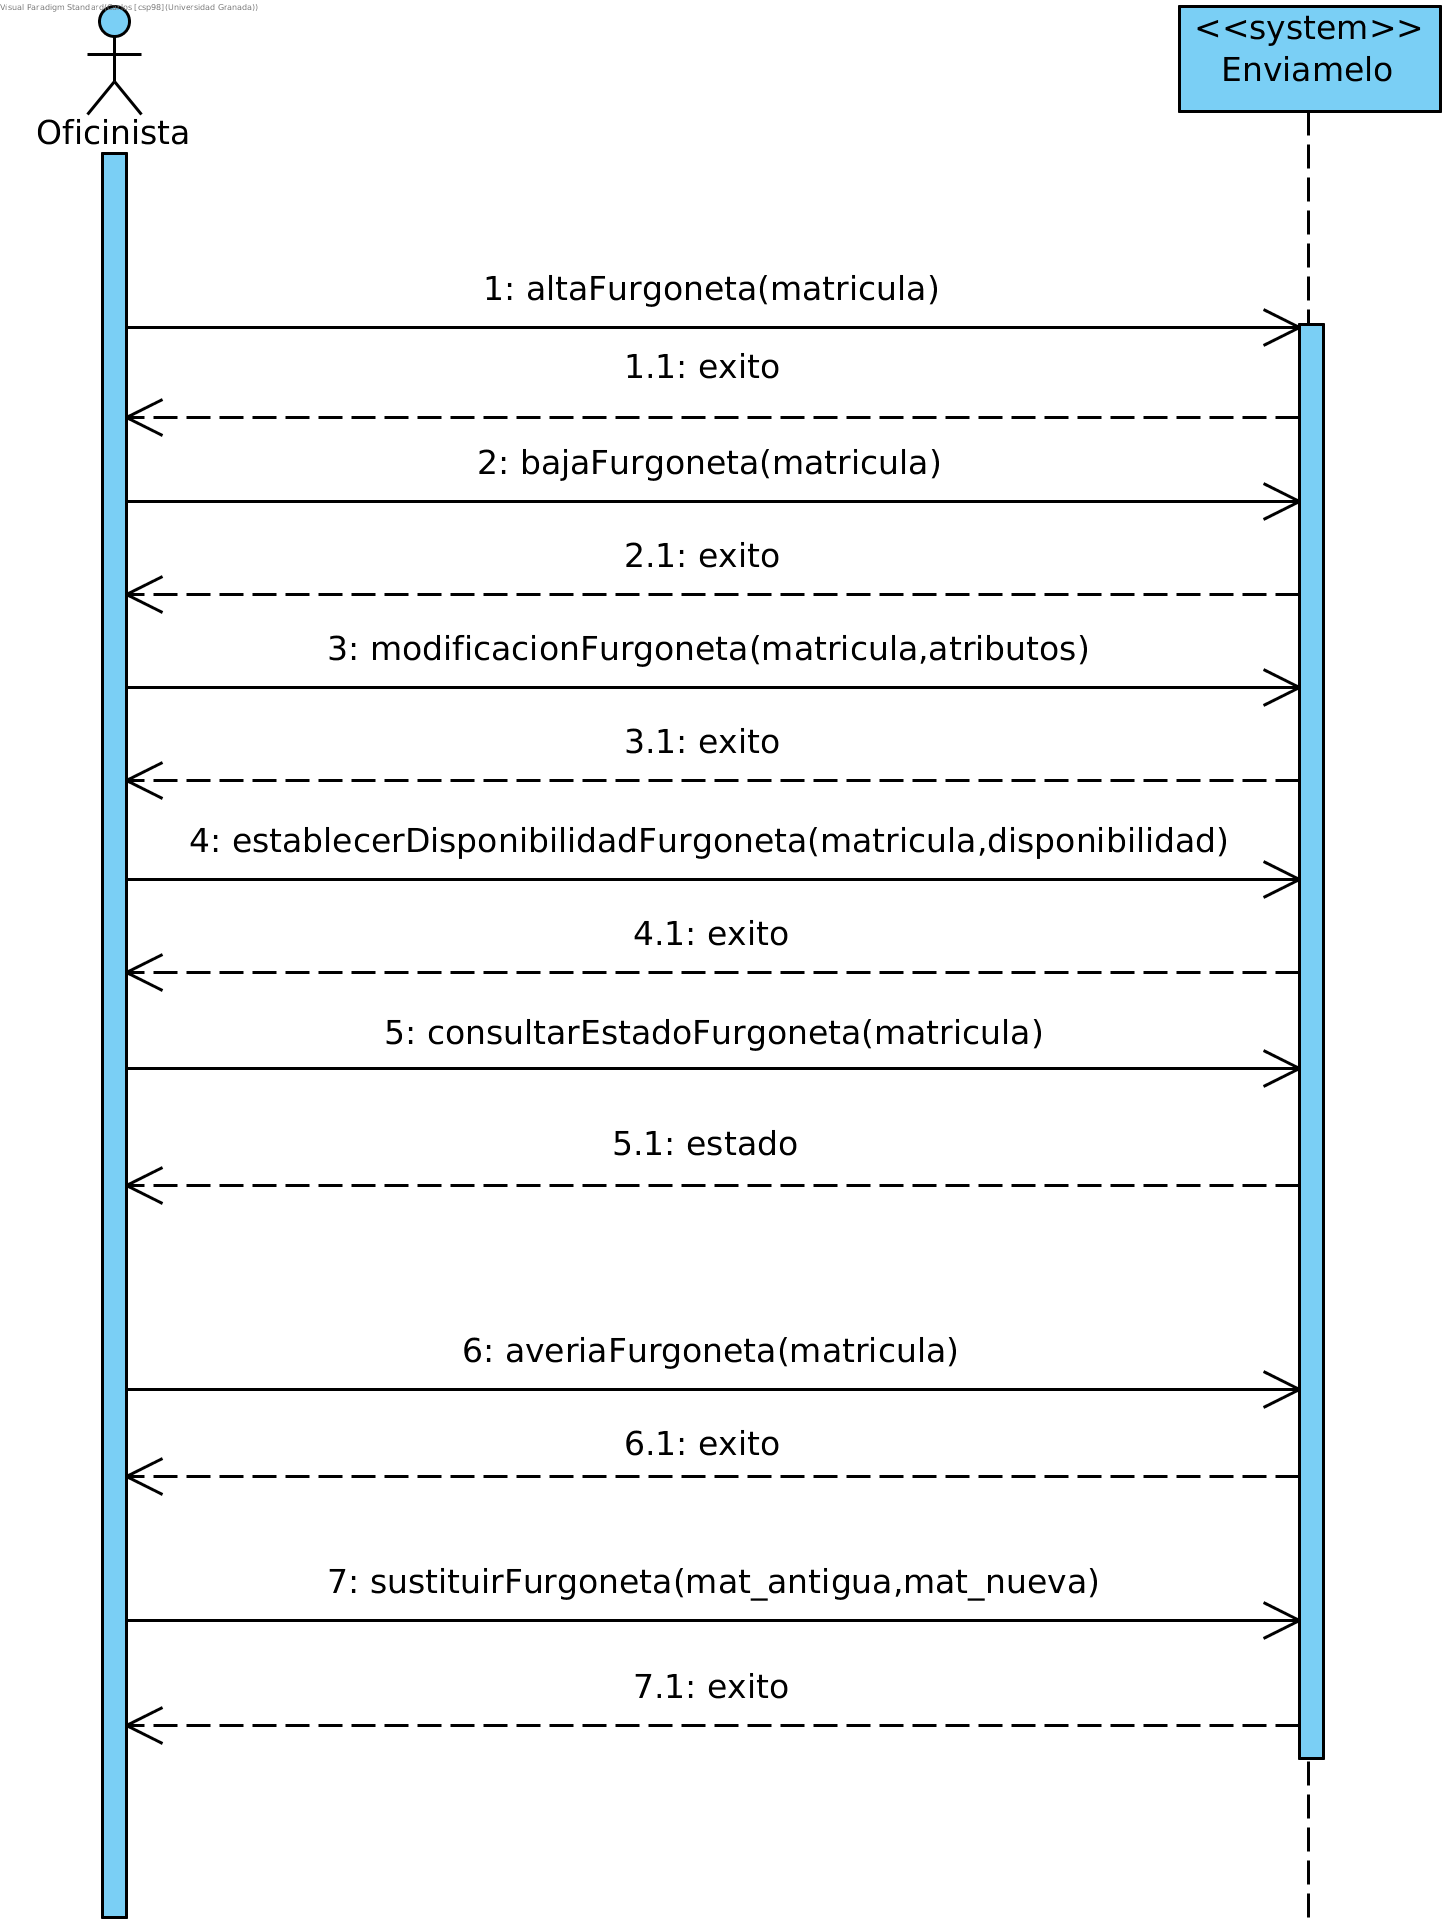
\includegraphics[scale=1]{gestion_flota.png}
\caption{Gestión de flota.}
\end{figure}

\begin{figure}[H]
\centering
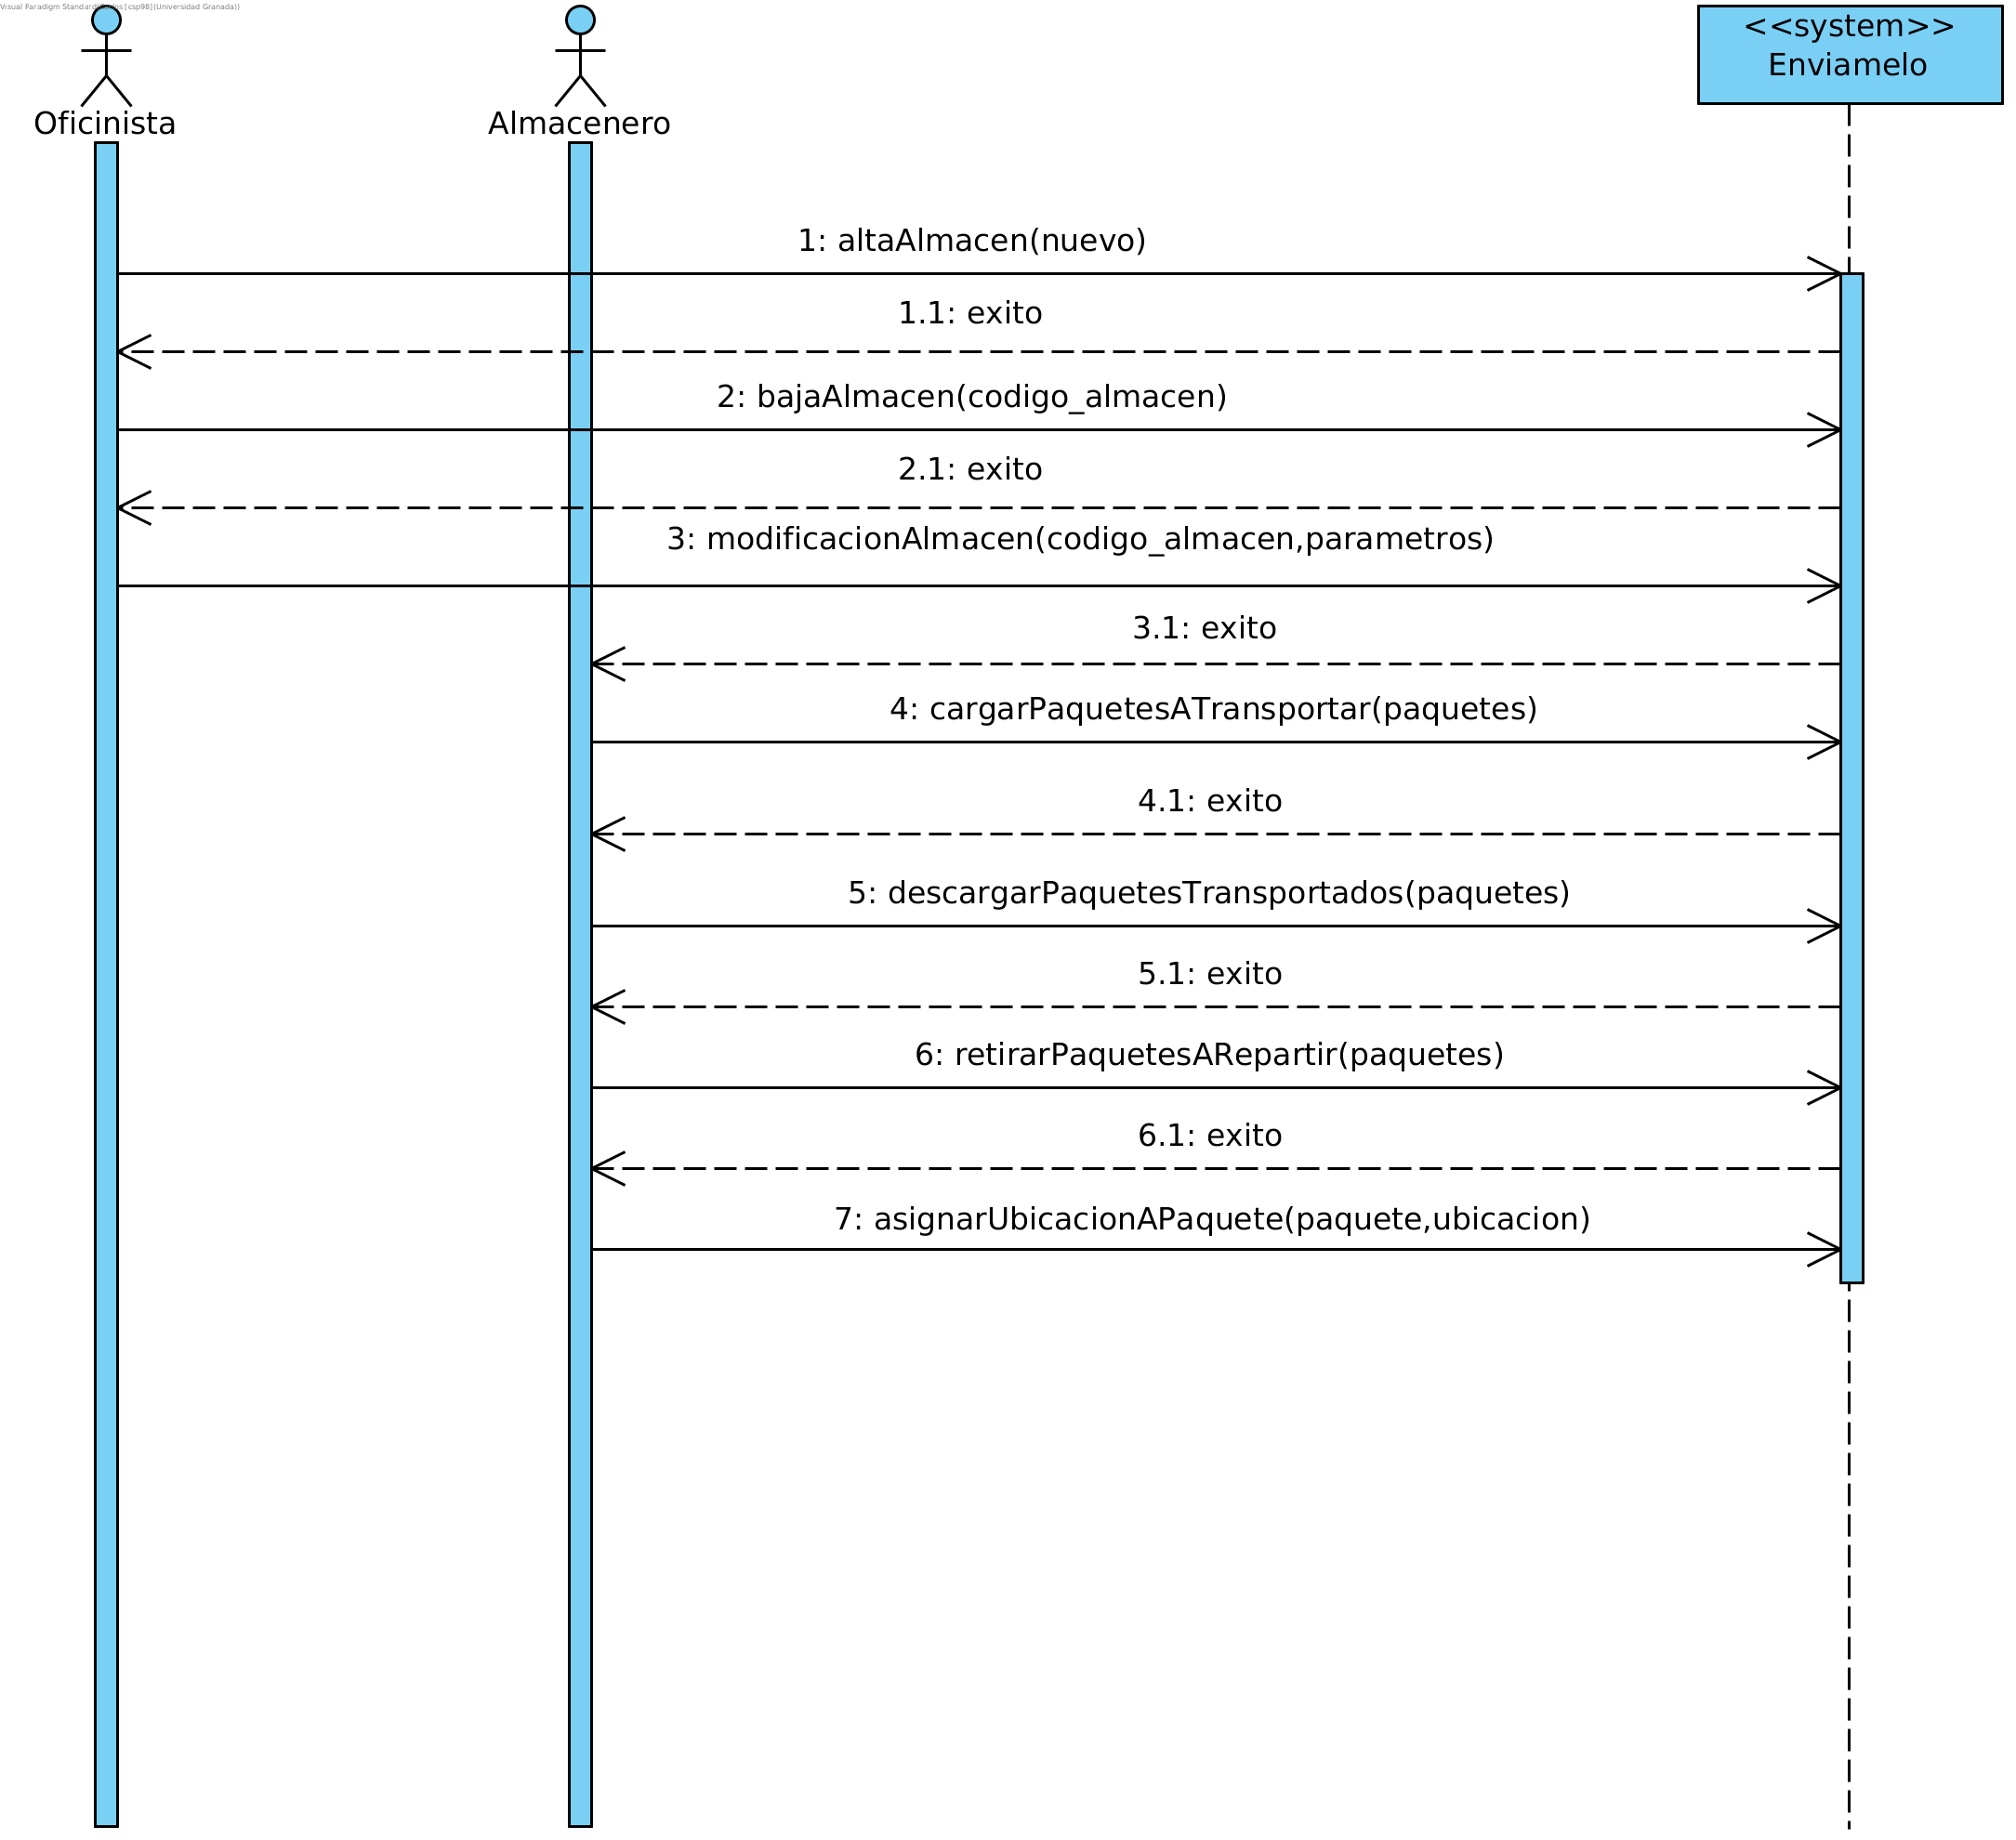
\includegraphics[scale=0.8]{gestion_almacen.png}
\caption{Gestión de almacén.}
\end{figure}

\begin{figure}[H]
\centering
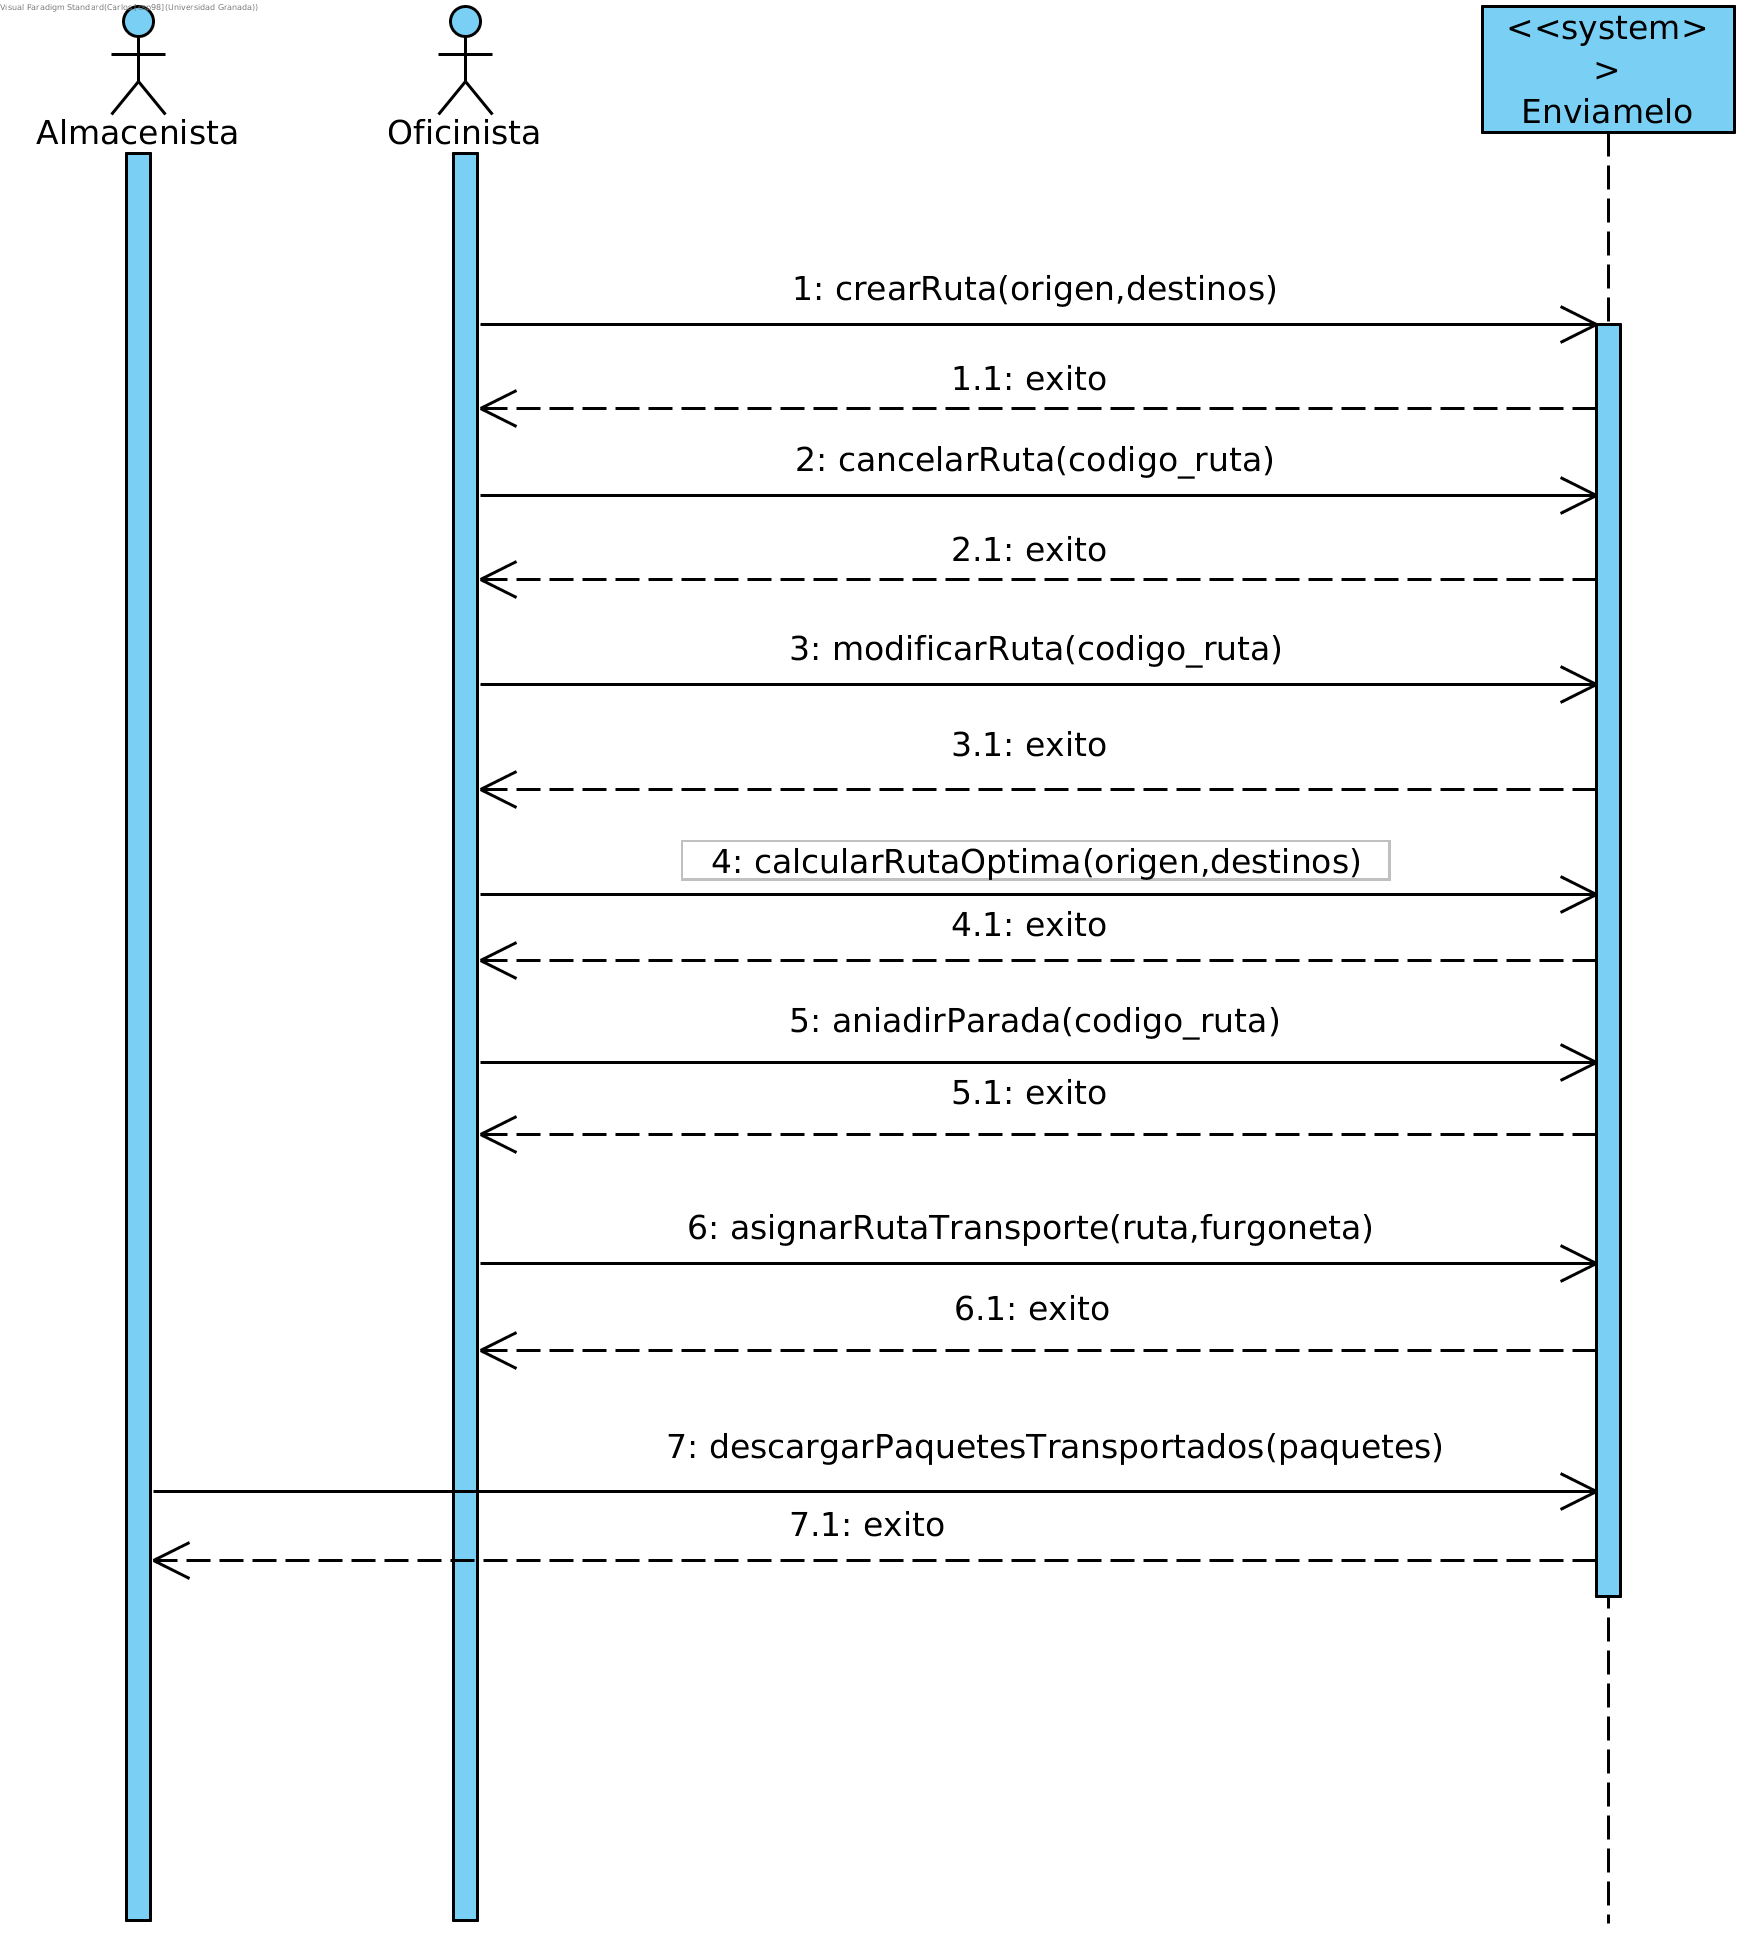
\includegraphics[scale=1]{gestion_transporte.png}
\caption{Gestión de transporte.}
\end{figure}

\begin{figure}[H]
\centering
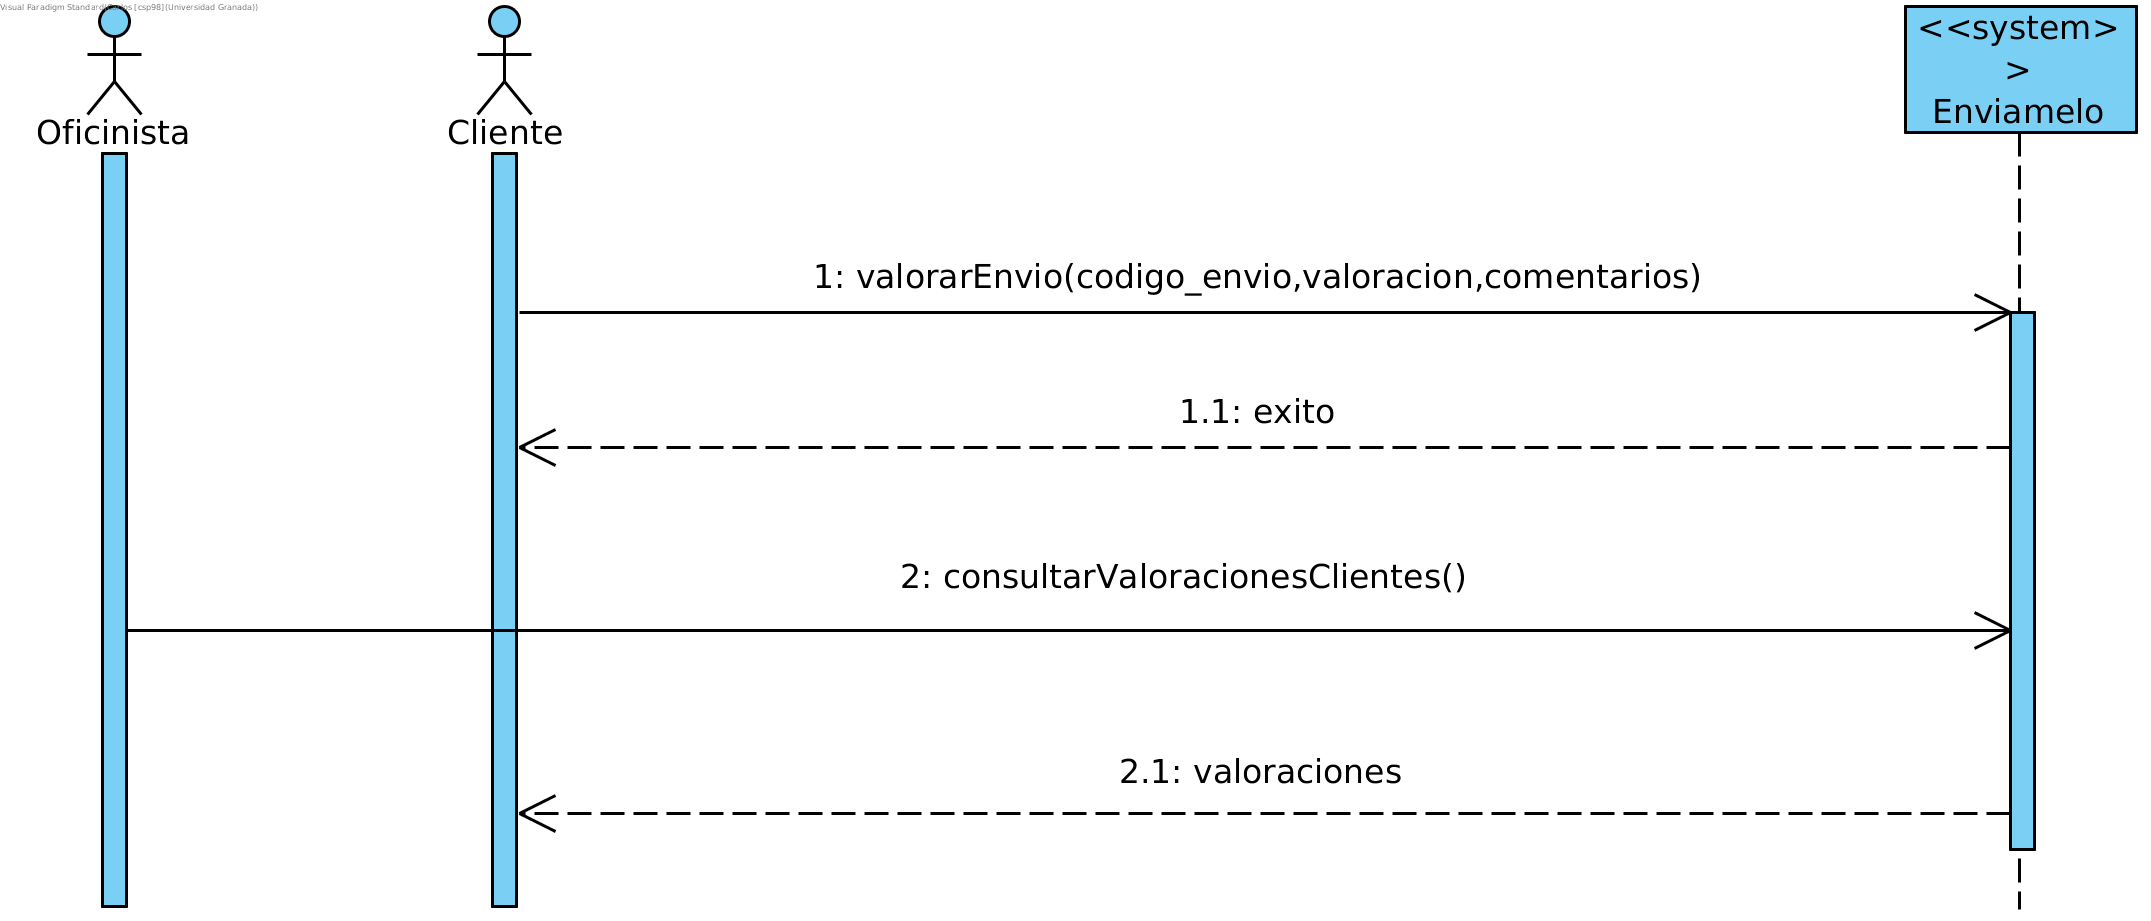
\includegraphics[scale=0.8]{atencion_cliente.png}
\caption{Atención al cliente.}
\end{figure}


%%%%%%%%%%%%%%%%%%%%%%%%%%%%Fin del documento%%%%%%%%%%%%%%%%%%%%%%%%%%%%%%%%%
\end{document}
